% LaTeX path to the root directory of the current project
\providecommand{\econtexRoot}{}
\renewcommand{\econtexRoot}{.}
\documentclass[../CGMPort.tex]{subfiles}
\onlyinsubfile{% https://tex.stackexchange.com/questions/463699/proper-reference-numbers-with-subfiles
    \csname @ifpackageloaded\endcsname{xr-hyper}{%
      \externaldocument{\econtexRoot/BufferStockTheory}% xr-hyper in use; optional argument for url of main.pdf for hyperlinks
    }{%
      \externaldocument{main}% xr in use
    }%
    \renewcommand\labelprefix{}%
    % Initialize the counters via the labels belonging to the main document:
    \setcounter{equation}{\numexpr\getrefnumber{\labelprefix eq:AAgg}\relax}% eq:AAgg is the last numbered equation in the main text; start counting up from there
}

\begin{document}

\section{Comparison with CGM}\label{sec:Comparison}

\begin{figure}
	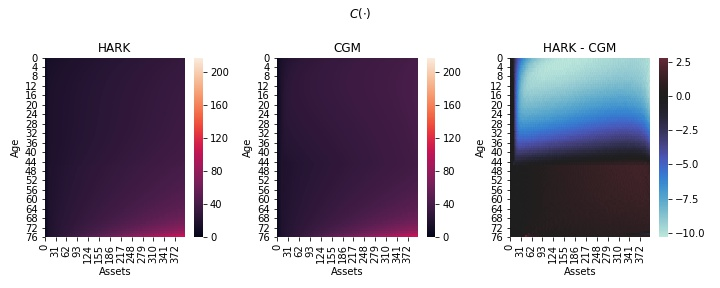
\includegraphics[width = \linewidth]{\FigDirPython/Cons_Pol_Compare}
	\caption{Consumption policy functions in HARK and CGM's Fortran code.}
\end{figure}

\begin{figure}
	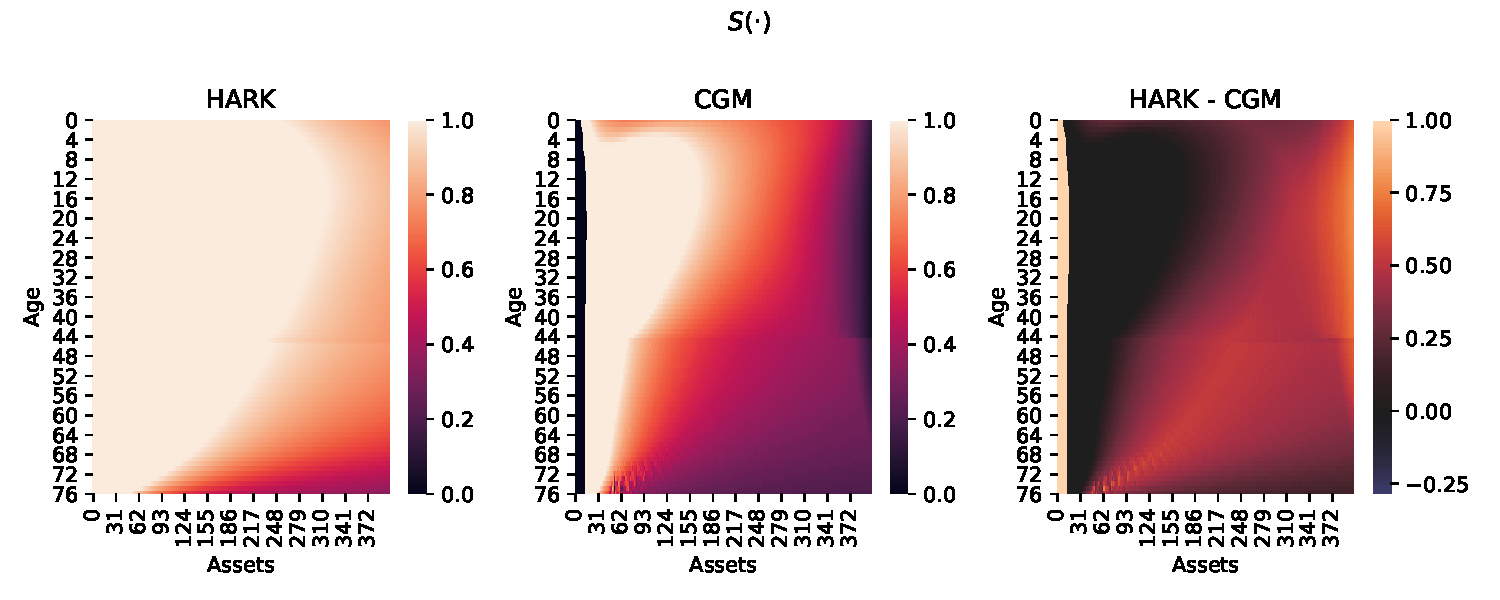
\includegraphics[width = \linewidth]{\FigDirPython/RShare_Pol_Compare}
	\caption{Risky share policy functions in HARK and CGM's Fortran code.}
\end{figure}

\begin{figure}
	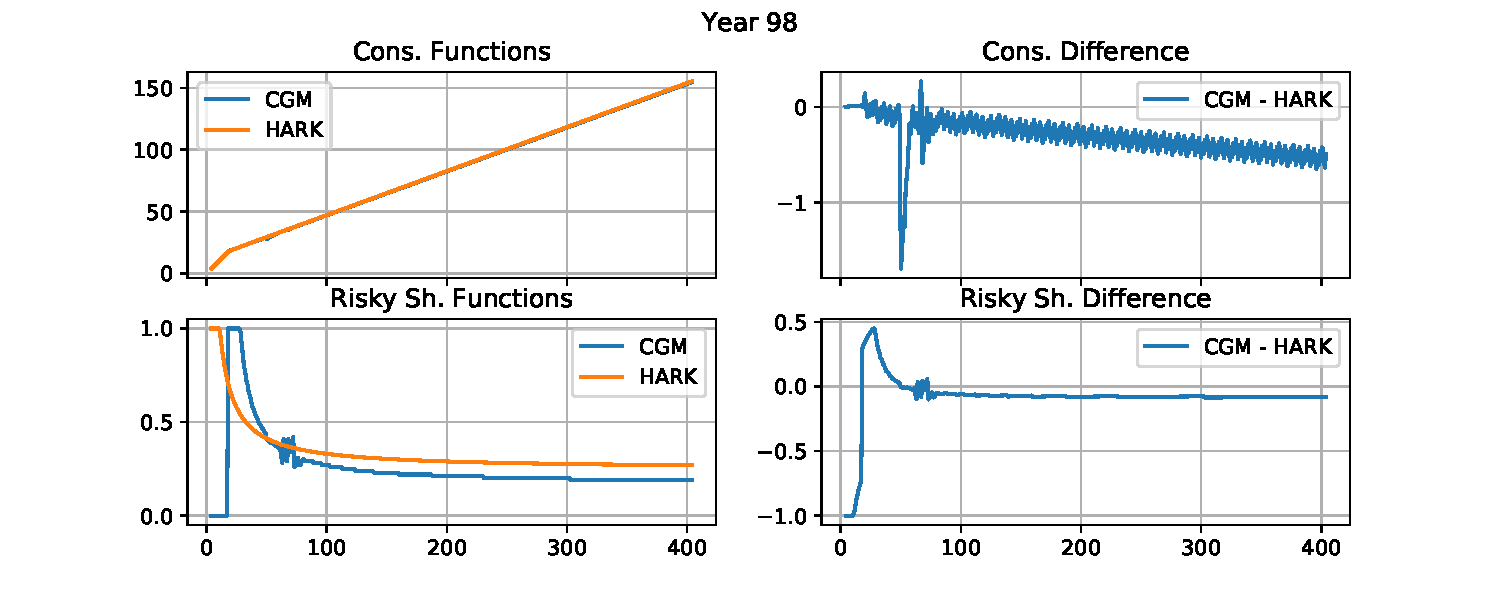
\includegraphics[width = \linewidth]{\FigDirPython/PolFunc_Compare_Y98}
	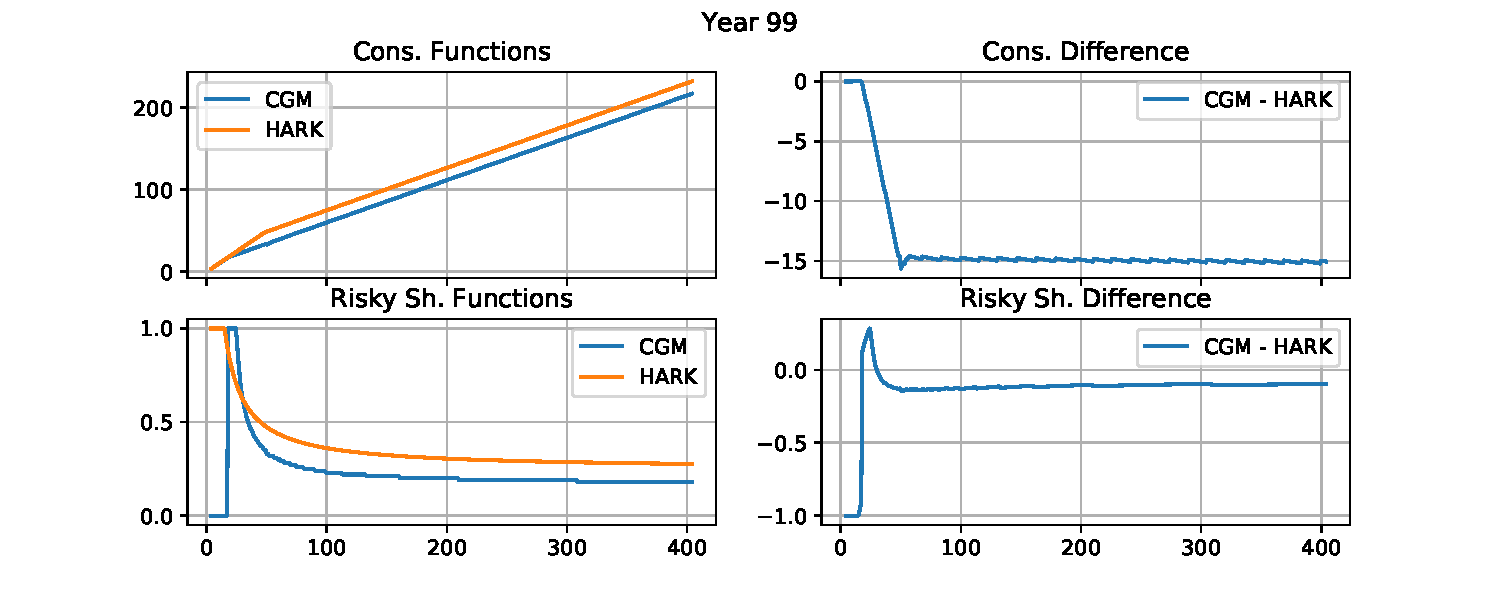
\includegraphics[width = \linewidth]{\FigDirPython/PolFunc_Compare_Y99}
	\caption{Policy functions in the second and third to last periods of life.}
\end{figure}

\section{Sensitivity analyses}\label{sec:Sensitivity}

Given that our main set of results does not align with the main article,
we provide a few tests that compare the behavior of the tools that we are using
with well known theoretical results.

\subsection{Merton Samuelson}

\begin{figure}
	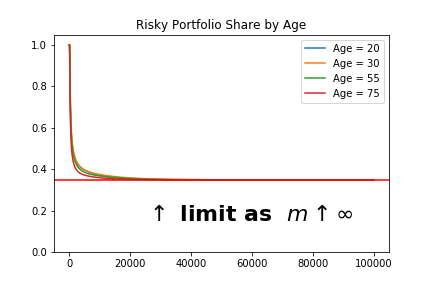
\includegraphics[]{\FigDirPython/Merton_Samuelson_Limit}
	\caption{Merton Samuelson as the limit of the risky asset's portfolio 
	share.}
\end{figure}

\subsection{Marginal Propensity to Consume}

\begin{figure}
	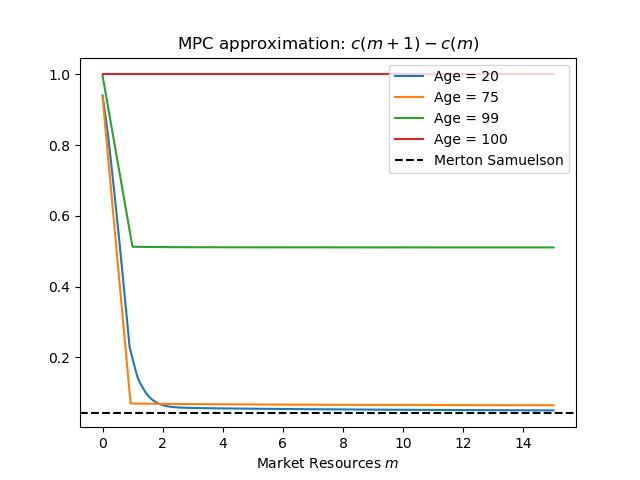
\includegraphics[]{\FigDirPython/MPC_Limit}
	\caption{Marginal propensity to consume as $m \rightarrow \infty$.}
\end{figure}

\subsection{Perfect Foresight and No Shocks}

\begin{figure}
	\includegraphics[]{\FigDirPython/Pf_Compare_Lvl}
	\caption{Perfect foresight solutions using different HARK tools.}
\end{figure}

\begin{figure}
	\includegraphics[]{\FigDirPython/Pf_Compare_Diff}
	\caption{Differences from the true Perfect foresight solution.}
\end{figure}

\end{document}
